\chapter{Resultados} \label{sec:results}

\section{Procesamiento de secuencias de ARN de tipo tallo-horquilla}

Se ha desarrollado una herramienta llamada HextractoR, simple e integrada, que automáticamente extrae y pliega todas las secuencias de horquilla a partir de
datos brutos del genoma completo. El método propuesto aprovecha los últimos avances en la predicción de estructuras secundarias. Al procesar grandes
ventanas superpuestas, no se pierden ni se cortan de manera inapropiada las horquillas. Permite procesar genomas en paralelo y con pocos requisitos de memoria,
ya que puede dividir automáticamente archivos fasta demasiado grandes.

Se procesaron varios genomas y los resultados se compararon con los del programa mirCheck de EMBOSS \citep{olson2002emboss}. La Tabla~\ref{tab:hextractor} muestra los
resultados del procesamiento de 6 genomas completos: \textit{Homo sapiens}, \textit{Arabidopsis thaliana}, \textit{Danio rerio}, \textit{Anopheles gambiae} y
\textit{Caenorhabditis elegans}, además de otra especie menos estudiada: \textit{Echinococcus multilocularis}. Para cada uno, se muestra el número de
secuencias extraídas con mirCheck y HextractoR, en la segunda y tercera columna, respectivamente. Con respecto a los pre-miARNs en particular se informa, en
cada genoma analizado, en la cuarta columna de la tabla el número de pre-miARNs conocidos (de acuerdo con miRBase 21) para las 6 especies. La proporción de
aquellos encontrados por los métodos comparativos se muestra en las dos últimas columnas. Se puede ver claramente que en todos los casos, el rendimiento de
HextractoR es superior. Además, en muchos casos, el 100 \% de los pre-miARNs conocidos se extraen correctamente.

Las diferencias en cantidad de pre-miARNs encontrados que muestra la Tabla~\ref{tab:hextractor} se pueden deber a varios motivos. En primer lugar, como se ve en
la segunda y tercer columna, HextractoR consigue capturar más horquillas que mirCheck. Al utilizar ventanas solapadas de un tamaño varias veces mayor al de
una horquilla para recorrer el genoma, HextractoR consigue capturar cualquier horquilla. MirCheck se podría configurar para que utilice ventanas con una mayor
longitud, pero en ese caso descartaría la mayoría de las secuencias porque estas formarían estructuras con varios bucles y mirCheck no realiza el proceso de
separación en horquillas como si lo hace HextractoR.

\begin{table}[t]
	\centering
	\small
	\begin{tabular}{l r r r r r c}
		\toprule
		\multirow{2}{*}{Especies} & \multicolumn{2}{c}{Horquillas extraídas}  & & \multicolumn{2}{c}{pre-miARNs encontrados}    &    pre-miARNs  \\ \cmidrule{2-3} \cmidrule{5-6}
						    &    Einverted  &       HExtractor     & & Einverted     &   HExtractor  &  conocidos \\ \cmidrule{1-7}
		\textit{Anopheles gambiae}          &  1.410.532    &  \textbf{4.276.543}  & &  92,42 \%     &    \textbf{100,00  \%}       &   66        \\
		\textit{Caenorhabditis elegans}     &    875.588    &  \textbf{1.739.124}  & &  90,00 \%     &     \textbf{99,60  \%}       &  250        \\
		\textit{Danio rerio}                & 11.028.128    & \textbf{23.214.338}  & &  93,06 \%     &     \textbf{99,42  \%}       &  346        \\
		\textit{Echinococcus multilocularis}&    509.530    &  \textbf{1.898.911}  & &  81,81 \%     &    \textbf{100,00  \%}       &   22        \\
		\textit{Arabidopsis thaliana}       &    874.320    &  \textbf{1.357.455}  & &  91,69 \%     &     \textbf{94,77  \%}       &  325        \\
		\textit{Homo sapiens}               & 18.654.426    & \textbf{48.206.494}  & &  85,38 \%     &     \textbf{97,45  \%}       & 1881        \\
		\bottomrule
	\end{tabular}
	\label{tab:hextractor}
	\caption[Cantidad de horquillas y pre-miARN en varios genomas]{cantidad de horquillas y pre-miARNs encontrados por cada método en el genoma de 6 especies}
\end{table}

\section{Predicción de pre-microARN}

En esta sección se presentan los resultados de los experimentos realizados para probar el rendimiento de miRNAss en diferentes condiciones. En la primera
subsección, se reprodujeron experimentos realizados por otros autores para comparar miRNAss con métodos supervisados del estado del arte en condiciones
controladas. Los conjuntos negativos fueron definidos artificialmente por los autores originales y la proporción de ejemplos etiquetados fue muy alta. En la
segunda subsección, el porcentaje de ejemplos etiquetados se redujo gradualmente para acercarse más a un caso real de predicción de pre-miARN. Además,
miRNAss se probó en un esquema de una clase, donde solo se conocían ejemplos positivos (pre-miARNs reales) de antemano. En la última subsección, miARN se
aplicó a una tarea de predicción real a partir de datos del genoma completo de 3 especies modelo, sin ejemplos negativos y utilizando solo un bajo número de
ejemplos positivos. En esta última prueba, había un enorme desbalance de clases y se procesaron más de un millón de secuencias de entrada.
Comparación en conjuntos de datos etiquetados artificialmente

\subsection*{Comparación con métodos del estado del arte}
Las condiciones experimentales en esta sección son las mismas que las utilizadas para probar otros métodos del estado del arte. Se estableció $ F_{1} $ como
medida de desempeño utilizada para la optimización del umbral en todos los métodos. Los experimentos se diseñaron para estimar el desempeño de métodos de
aprendizaje supervisado, por lo que se utiliza un esquema estándar de validación cruzada con 10 particiones. En este esquema, la mayoría de las secuencias
están etiquetadas artificialmente para el entrenamiento, y solo un $ 10 \% $ queda sin etiquetar. Por lo tanto, es importante señalar que la principal
ventaja del aprendizaje semi-supervisado, que es explotar datos no etiquetados para mejorar los resultados, no se puede aprovechar en estos experimentos.
Para una comparación justa, en estos experimentos los clasificadores usan las mismas características. Este conjunto está compuesto por 7 características de
miPred \citep{ng2007novo}, más 14 de microPred \citep{batuwita2009micropred} y 7 añadidas por \cite{gudys2013huntmi}. Para obtener más detalles sobre el
conjunto de características, consulte la Sección S4 del Anexo~\ref{sec:mirnass}.

Como antes se especificó, se ejecutó una validación cruzada estratificada de 10 particiones en cinco conjuntos de datos y se compararon los resultados con
los obtenidos por HuntMi \citep{gudys2013huntmi}. Las particiones fueron construidas al azar usando una semilla fija para tener experimentos totalmente
reproducibles. Tres conjuntos de datos contenían una mezcla de secuencias de diferentes especies, que se agruparon en los conjuntos de datos animales (10
especies), plantas (7 especies) y virus (29 especies). Los otros dos conjuntos de datos contenían secuencias de \textit{Homo sapiens} y \textit{Arabidopsis
thaliana}. Los parámetros utilizados en miRNAss fueron los mismos en todas las pruebas: $ c = 1 $ y $ k = 10 $ (tanto para RELIEF-F como para la construcción
de grafos). MiRNAss se probó con y sin RELIEF-F, para medir su impacto en el rendimiento. La ponderación de características obviamente se calculó
utilizando solo los datos de entrenamiento de cada partición.


Los tiempos transcurridos medidos \footnote{Intel \textregistered Core \texttrademark i5-4460 CPU @ 3.20GHz, 8 GB de RAM.} En cada pliegue se promediaron y se
presentan en la Tabla~\ref{tab:times}. La primera columna muestra el número total de secuencias. La segunda y tercera columnas indican el número de
secuencias pre-miARN y no pre-miARN en cada conjunto de datos. La cuarta y quinta columnas presentan los tiempos transcurridos para cada método. La última
columna muestra el cociente entre el tiempo que tardó HuntMi y el tiempo que tardó miRNAss. La mayor diferencia se observó en el conjunto de datos más
pequeño (virus): miRNAss fue 38 veces más rápido que HuntMi. Arabidopsis es el segundo conjunto de datos más pequeño, y aquí miRNAss fue 14 veces más
rápido. En los siguientes tres conjuntos de datos, las diferencias de tiempo de computación entre miRNAss y HuntMi aumentaron a medida que crecía el número
de secuencias. Estos resultados muestran que miARN no solo es mucho más rápido sino que el costo computacional crece más rápido en HuntMi. Tales
diferencias pueden ser irrelevantes en pequeños conjuntos de datos como los que se utilizan en esta subsección, pero se vuelven muy importantes en tareas de
predicción de genoma completo, donde se procesan varios millones de secuencias. Por ejemplo, si extrapolamos los tiempos de entrenamientos utilizando los
datos de la tabla, para entrenar a HuntMi con 1.7 millones de secuencias (uno de los conjuntos de datos del genoma utilizado en la sección~\ref{sec:results:genome-wide})
se necesitarían alrededor de 37 días, mientras que miRNAss solo se requieren 18 horas.
Con respecto a las medidas de predicción, ambos métodos se realizaron de manera similar en este experimento. Se aplicó una prueba de Friedman \citep{friedman1937use},
que dio como resultado un valor $ p $ de 0,179. Esto demuestra que el método propuesto puede obtener resultados equivalentes a un método
del estado del arte para la configuración supervisada, aunque en menos tiempo (como se muestra en la Tabla~\ref{tab:times}).
\begin{table}[t]
	\small
	\centering
	\begin{tabular}{@{}lrrrrrrr@{}} \toprule
		&  \multicolumn{3}{c}{Número de secuencias} & & \multicolumn{3}{c}{Tiempos} \\ \cmidrule{2-4} \cmidrule{6-8}
		Conjunto de datos     &   Total  &   miARN   &  no-miARN& &  HuntMi  & miRNAss & \textit{speedup} \\\midrule
		Virus       &   1,076  &      237  &       839 & &     38 s &     1 s & 38.00    \\
		Arabidopsis &  28,590  &      231  &    28,359 & &  1,819 s &   129 s & 14.10    \\
		Human       &  82,634  &    1,406  &    81,228 & &  9,873 s &   462 s & 21.37    \\
		Plants      & 117,101  &    2,172  &   114,929 & & 21,561 s &   714 s & 30.19    \\
		Animals     & 225,207  &    7,053  &   218,154 & & 65,762 s & 1,834 s & 35.85    \\\bottomrule
	\end{tabular}
	\caption[Comparación de tiempos de ejecución]{comparación de los tiempos de ejecución entre miRNAss y HuntMi.\label{tab:times}}
\end{table}
Además, fue posible verificar que RELIEF-F mejoró los resultados en todas las pruebas, aunque en algunas de ellas las diferencias fueron pequeñas. Esto era
de esperar, dado que las características utilizadas en estos conjuntos de datos son el resultado de procesos previos de selección de características. Una
prueba de Friedman en esta comparación da como resultado un valor $ p $ de 0.025, lo que demuestra que las diferencias son significativas. Se pueden ver más
detalles sobre estos resultados en la Figura~S5 del Anexo~\ref{sec:mirnass}.

Para probar la capacidad de miRNAss para predecir nuevos pre-miARNs en diferentes especies, los pre-miARNs conocidos de animales y plantas que se incluyeron en
la versión 17 de mirBase se usaron para el entrenamiento, y los pre-miARNs que se agregaron en versiones 18 a 19 fueron usados como conjunto de prueba. En el caso de las especies
animales, se añadió microPred \citep{batuwita2009micropred} en la comparación, ya que era el mejor software para la predicción de miARN humano en el
momento de su publicación. En plantas, el método agregado fue PlantMiRNAPred \citep{xuan2011plantmirnapred}, porque está específicamente diseñado para
especies de plantas. Cabe señalar que, una vez más, el porcentaje de secuencias no etiquetadas en el conjunto de datos es muy bajo: menos del 0,3 \% en
animales y menos del 1,3 \% en plantas.
\begin{figure}[t]
	\centering
	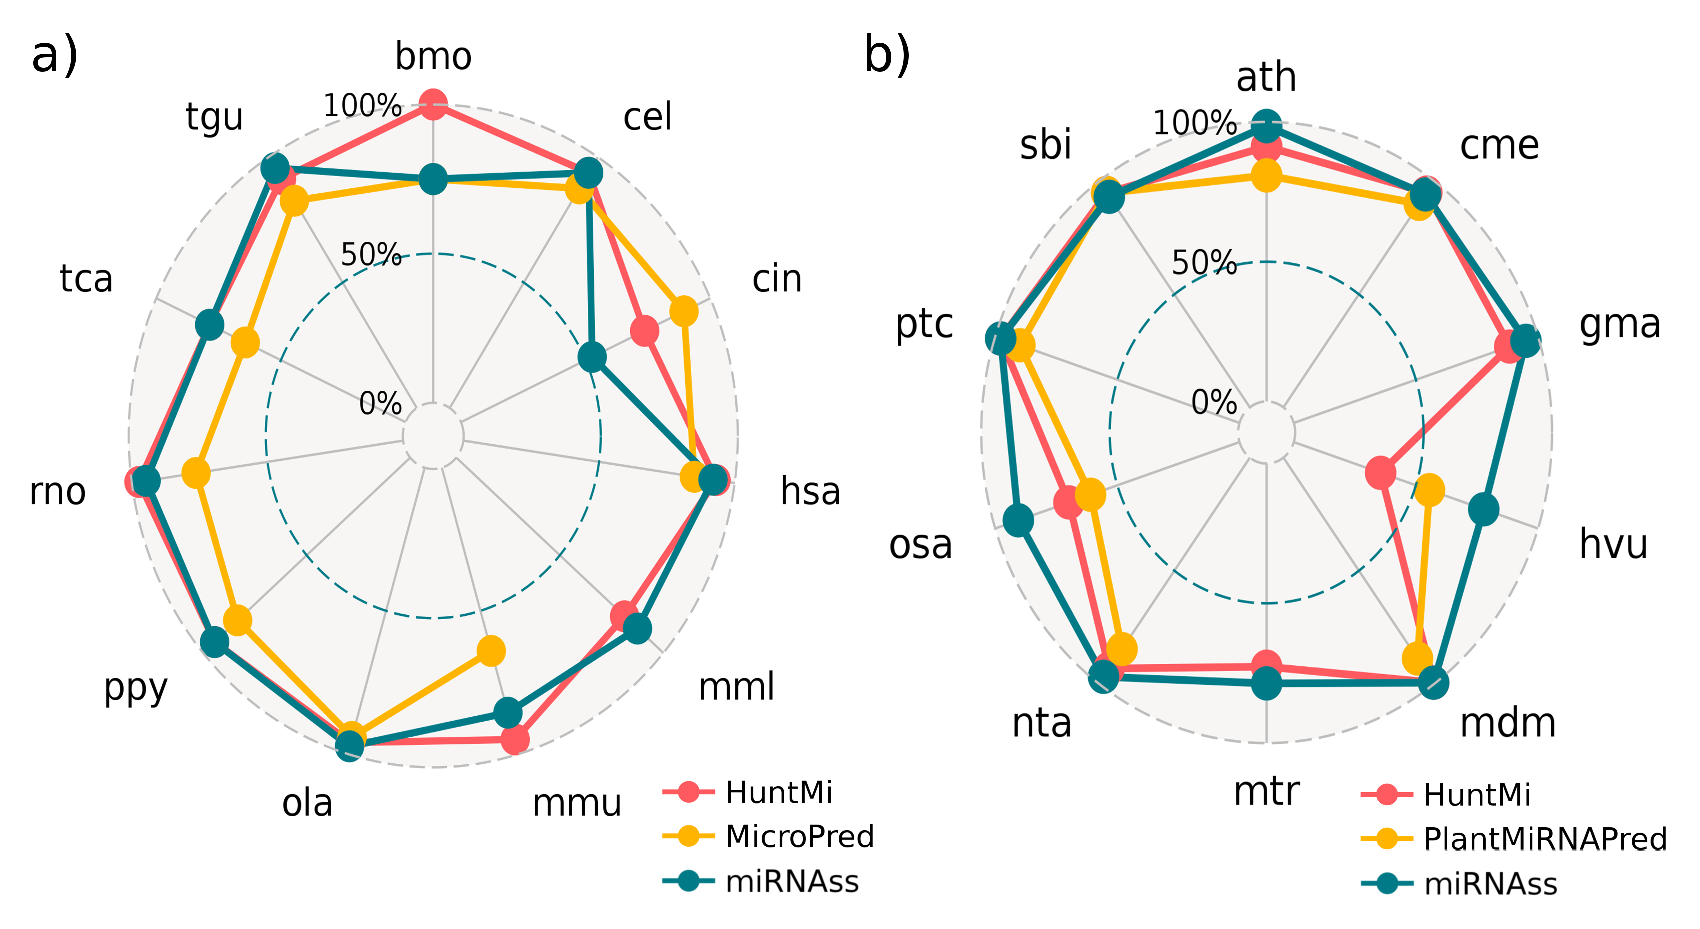
\includegraphics[width=0.6\linewidth]{fig/delta_mirbase_radar.eps}
	\caption[Sensibilidad en animales y plantas]{sensibilidad obtenida con varios clasificadores del estado del arte en: a) animales, y b) plantas.
		La distancia de cada punto al centro mide la sensibilidad obtenida obtenida cada especie.}
	\label{fig:deltaRadar}
\end{figure}
La $S^{+}$ obtenida para cada especie se muestran en la Figura~\ref{fig:deltaRadar}, donde cada clasificador se muestra con un color diferente a través de una
gráfica de radar. En el conjunto de datos de animales, miRNAss superó a microPred en casi todas las especies. En el conjunto de datos humanos, miRNAss obtuvo
una mayor $S^{+}$ que microPred, que, como se mencionó anteriormente, se diseñó específicamente para humanos. Comparado con HuntMi, miRNAss obtuvo mayores
$S^{+}$ en 4 especies, HuntMi produjo mejores resultados en 4 especies y los resultados obtenidos fueron iguales en 3 especies. En plantas, miRNAss superó a
PlantMiRNAPred en casi todas las especies. Comparado con HuntMi, miRNAss tuvo una mejor $S^{+}$ en 8 especies, mientras que HuntMi superó ligeramente al
miRNAss en solo 2 especies (\textit{Cucumis melo} y \textit{Sorghum bicolor}).
Para analizar si hubo diferencias significativas entre los clasificadores, se realizaron pruebas de Nemenyi \citep{nemenyi1962distribution} para ambos
conjuntos de datos ($ p<0,05 $). En las especies de animales, HuntMi y miRNAss produjeron resultados equivalentes, pero ambos se desempeñaron mejor que
microPred. En especies de plantas, miRNAss obtuvo el rango más bajo (el mejor) y una diferencia significativa con PlantMiRNAPred. Sin embargo, la diferencia
con HuntMi no fue estadísticamente significativa.

Los métodos supervisados hacen un uso extenso de los datos etiquetados, no solo para el entrenamiento sino también para encontrar los hiper-parámetros
y umbrales óptimos. Por el contrario, miRNAss se diseñó sobre la hipótesis de que los ejemplos etiquetados son escasos, poco confiables y no
representativos de toda la clase, que en realidad es un escenario más realista para esta tarea de predicción. Por lo tanto, debe tenerse en cuenta que,
incluso bajo estas condiciones desfavorables, miRNAss obtuvo resultados significativamente mejores que MicroPred y PlantMiRNAPred, y resultados equivalentes a
los producidos por HuntMi, siendo sin embargo, mucho más rápido.

\subsection*{Pocos ejemplos etiquetados}

\begin{figure}[t]
	\centering
	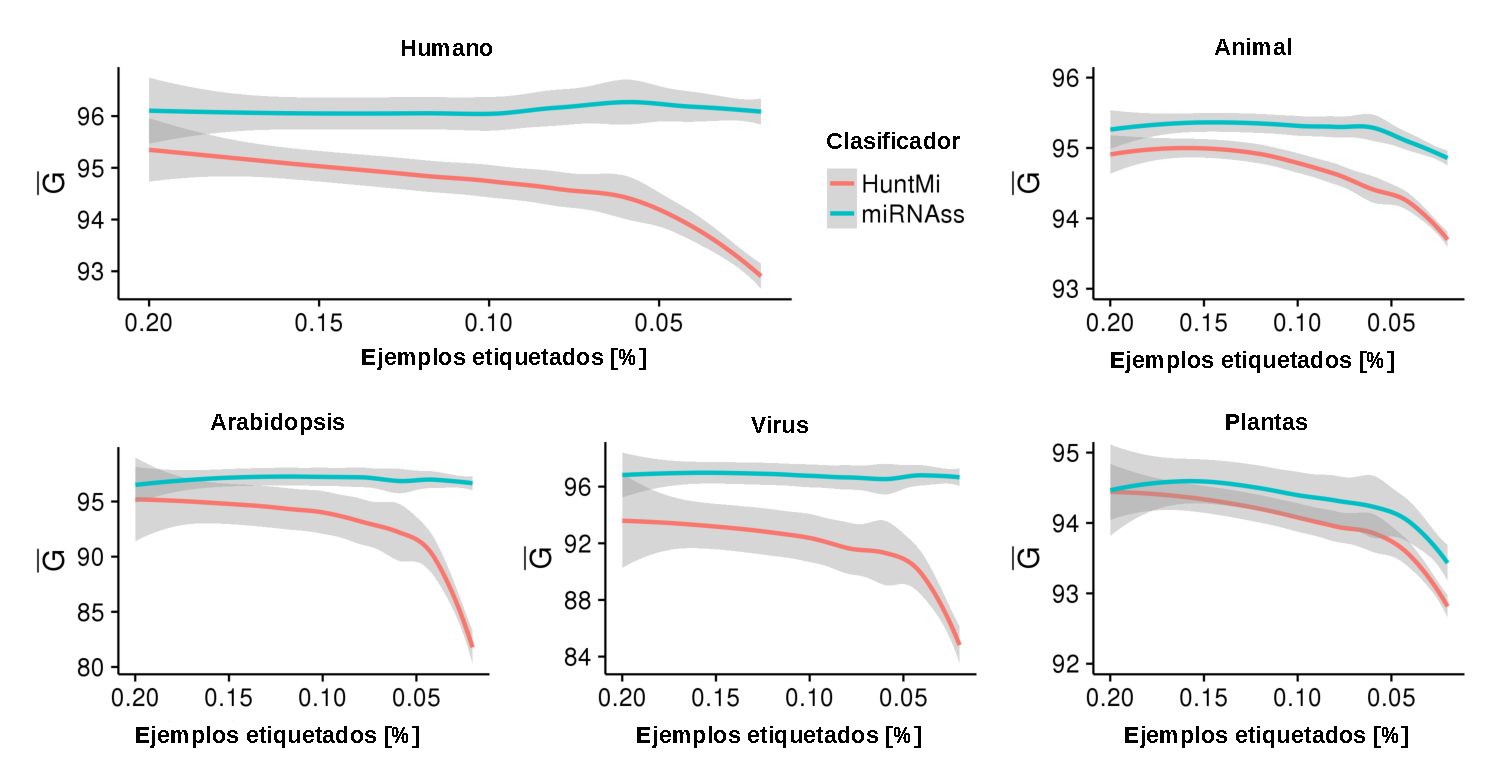
\includegraphics[width=\linewidth]{fig/few_labeled-huntmi.eps}
	\caption[$\bar{G}$ con pocos ejemplos de entrenamiento]{curvas de $\bar{G}$ obtenidas al disminuir el porcentaje de ejemplos etiquetados. Regiones
		sombreados representan los intervalos de confianza de la estimación con regresión local (LOESS) con $p < 0.05$.}
	\label{fig:fewSamples:huntmi}
\end{figure}

Para representar un escenario más realista en el que el número de ejemplos conocidos es bajo, los cinco conjuntos de datos utilizados en las últimas pruebas
se utilizaron con distintos porcentajes de secuencias etiquetadas y se realizaron pruebas en un esquema de validación entrenamiento-prueba. El porcentaje de
ejemplos etiquetados se redujo del 20 \% al 2 \%, con un paso del 2 \%. Los ejemplos etiquetados se seleccionaron al azar y las pruebas se repitieron 200 veces
para cada porcentaje para estimar los intervalos de confianza. En la Figura~\ref{fig:fewSamples:huntmi}, se estimaron las curvas de $F_{1}$ esperadas con
intervalos de confianza de 0,05 para la comparación. En el conjunto de datos humanos, el $F_{1}$ es casi un 10 \% más alto para miRNAss, independientemente
del porcentaje de secuencias marcadas. En el conjunto de datos de Arabidopsis, donde el número de secuencias de ejemplos positivos fue menor, las diferencias
a favor de miRNAss fueron más altas en los porcentajes más bajos de ejemplos etiquetados, lo que indica que miRNAss puede identificar efectivamente la clase
positiva incluso con un número muy bajo de ejemplos. Las mismas tendencias se observan en los animales, las plantas y los conjuntos de datos de virus.
Estos resultados no solo muestran que miRNAss es capaz de superar a los métodos supervisados cuando el número de ejemplos etiquetados es bajo, sino
también que las tasas de error estimadas usando una alta proporción de ejemplos etiquetados son muy diferentes de las obtenidas en escenarios más realistas.

Un paso más hacia una tarea de predicción más realista consiste en usar solo ejemplos positivos. Bajo estas condiciones, miRNAss se comparó con miRank
\citep{xu2008microrna}, que fue diseñado para trabajar con un número extremadamente pequeño de ejemplos positivos. Se utilizaron los conjuntos de datos
proporcionados por el autor original: 533 pre-miARNs humanos y 1000 secuencias no miARN. Para hacer una comparación justa, ambos métodos usaron el conjunto
de características de miRank. Este conjunto está compuesto por 32 tripletas \citep{xue2005classification}, MFE normalizado, propensiones de emparejamiento de
bases normalizadas de ambos brazos y longitud de bucle normalizado. Se marcó un número variable de ejemplos positivos (1, 2, 4, 8, 16, 32, 64 y 128) y el
resto de las secuencias se dejaron sin etiquetar para medir las tasas de error. Como los resultados dependen de un muestreo aleatorio de las secuencias, este
procedimiento se repitió 1000 veces para cada número de ejemplos etiquetados. MiRank proporciona como resultado una puntuación continua; por lo tanto, se
utilizaron los puntajes de predicción obtenidos con miRNAss en lugar de utilizar las clases. Se calculó el área bajo la curva de precisión-recuperación
(AUCPR, del ingles \textit{Area Under Precision-Recall Curve}), para realizar una comparación independiente del umbral utilizado para definir las clases
\citep{bradley1997use}.
La figura~\ref{fig:miRank} presenta un diagrama de caja con la distribución de AUCPR obtenida por cada clasificador para diferentes cantidades de ejemplos
etiquetados. MiRNAss mantuvo una AUCPR casi constante, independientemente del número de pre-miARNs marcados, mientras que el rendimiento de miRank disminuyó
marcadamente. Además, los valores de AUCPR para miRNAss mostraron pequeña dispersión en comparación con miRank, que se vuelve muy inestable cuando
disminuye el número de ejemplos etiquetados. Esta inestabilidad puede ser producida por ejemplos positivos que están cerca de la frontera de la clase, lo que
hace que miRank no establezca correctamente la frontera de decisión. El algoritmo semi-supervisado de miRNAss logró encontrar correctamente las regiones de
baja densidad que separan los miARNs del resto de las secuencias, independientemente de los ejemplos proporcionados.

\begin{figure}[tpb]
	\centering
	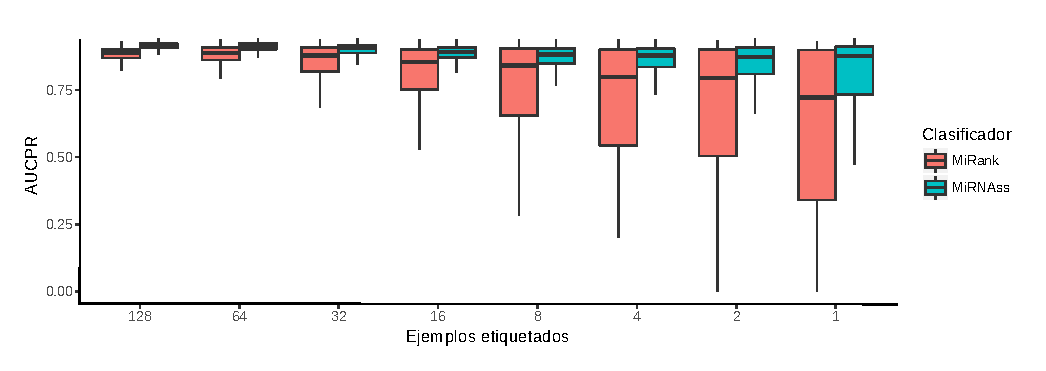
\includegraphics[width=\linewidth]{fig/few_samples_miRank.eps}
	\caption[$AUC$ con pocos ejemplos positivos]{diagrama de caja de las AUC obtenidas por miRNAss y miRank, con diferentes cantidades de ejemplos de entrenamiento positivos.}
	\label{fig:miRank}
\end{figure}

\subsection*{Predicción real en genomas completos} \label{sec:results:genome-wide}

MiRNAss se probó con los datos genómicos de tres genomas bien conocidos: \textit{Arabidopsis thaliana}, \textit{Caenorhabditis elegans} y \textit{Anopheles
gambiae}, para reproducir todas las condiciones de una tarea de predicción real. Los genomas completos se procesaron para extraer todos las secuencias con
estructura secundaria tipo tallo-horquilla existentes. Para este propósito se utilizó HExtractor, la herramienta desarrollada para tal fin. Este proceso
dejó un total de 1.356.616 secuencias de \textit{A. thaliana}; 1,698,859 secuencias de \textit{C. elegans}; y 4,276,188 secuencias de \textit{A. gambiae}.
Para detectar los pre-miARNs conocidos se utilizó la base de datos mirBase v21. Esto definió un total de 304, 249 y 66 horquillas como conjunto positivo para
\textit{A. thaliana}, \textit{C. elegans}, \textit{A. gambiae}, respectivamente.
Se extrajeron dos conjuntos de características de los tres genomas. El primero (FS1) es el mismo usado en la Sección ~\ref{sec:results}.1, para hacer una
comparación justa con uno de los métodos. El segundo conjunto de características (FS2) es un conjunto ampliado compuesto por casi todas las características
propuestas para la predicción pre-miARN en la literatura. FS2 se calculó con miRNAfe y cada vector de característica resultó en 79 elementos. Para obtener más
información sobre los conjuntos de características, consulte la Sección~S4 del Anexo~\ref{sec:mirnass}. Se utilizó un esquema de validación cruzada (CV) de 10
veces para medir el rendimiento de miARNs con curvas ROC promediadas.
Muchos algoritmos de predicción pre-miARN se probaron en estos conjuntos de datos para comparar su rendimiento con miRNAss. En total se han probado once
predictores, pero la mayoría han fallado con datos genómicos o sus servidores no funcionan. Los cinco predictores que se pudieron aplicar a genomas completos
fueron HuntMi, Mirident \citep{liu2012integrated}, HHMMiR \citep{kadri2009hhmmir}, MiRPara \citep{wu2011mirpara} y miR-BAG \citep{jha2012mirbag}. Los primeros
dos métodos producen clasificaciones duras (en vez de puntajes continuos) por lo que se representan como puntos en las figuras ROC. Por otro lado, dado que
MiRPara, miR-BAG, HHMMiR y miARN proporcionan puntajes continuos, se dibujaron curvas ROC completas. MiR-BAG no se ejecutó en \textit{A. thaliana} porque no
proporciona un modelo pre-entrenado para plantas. Los puntajes de salida obtenidos con este método sólo pueden tomar cuatro valores posibles, por lo que las
curvas ROC contienen regiones constantes. Estos resultados se presentan en la Figura~\ref{fig:ROC}.

En el genoma de \textit{A. thaliana}, se puede ver que las curvas ROC de miRNAss están por encima de las curvas de miRPara y HHMMiR para todos los valores
umbral. Cabe señalar que Mirident, a pesar de tener la mayor tasa de positivos verdaderos (sensibilidad), también tiene la mayor tasa de falsos positivos.
HuntMi es más equilibrado, con un alto reconocimiento de secuencias positivas y un número moderado de falsos positivos. Sin embargo, está debajo de miRNAss
con cualquiera de los dos conjuntos de características.
En el genoma de \textit{C. elegans}, se puede hacer un análisis similar para HuntMi y Mirident. En este conjunto de datos, miR-BAG genera una curva ROC
similar a la curva de MiRPara, ambas debajo del resto de las curvas. HHMMiR presenta un mejor rendimiento que estos métodos, pero una vez más es superado por
miRNAss.
\begin{figure*}[tpb]
	\centering
	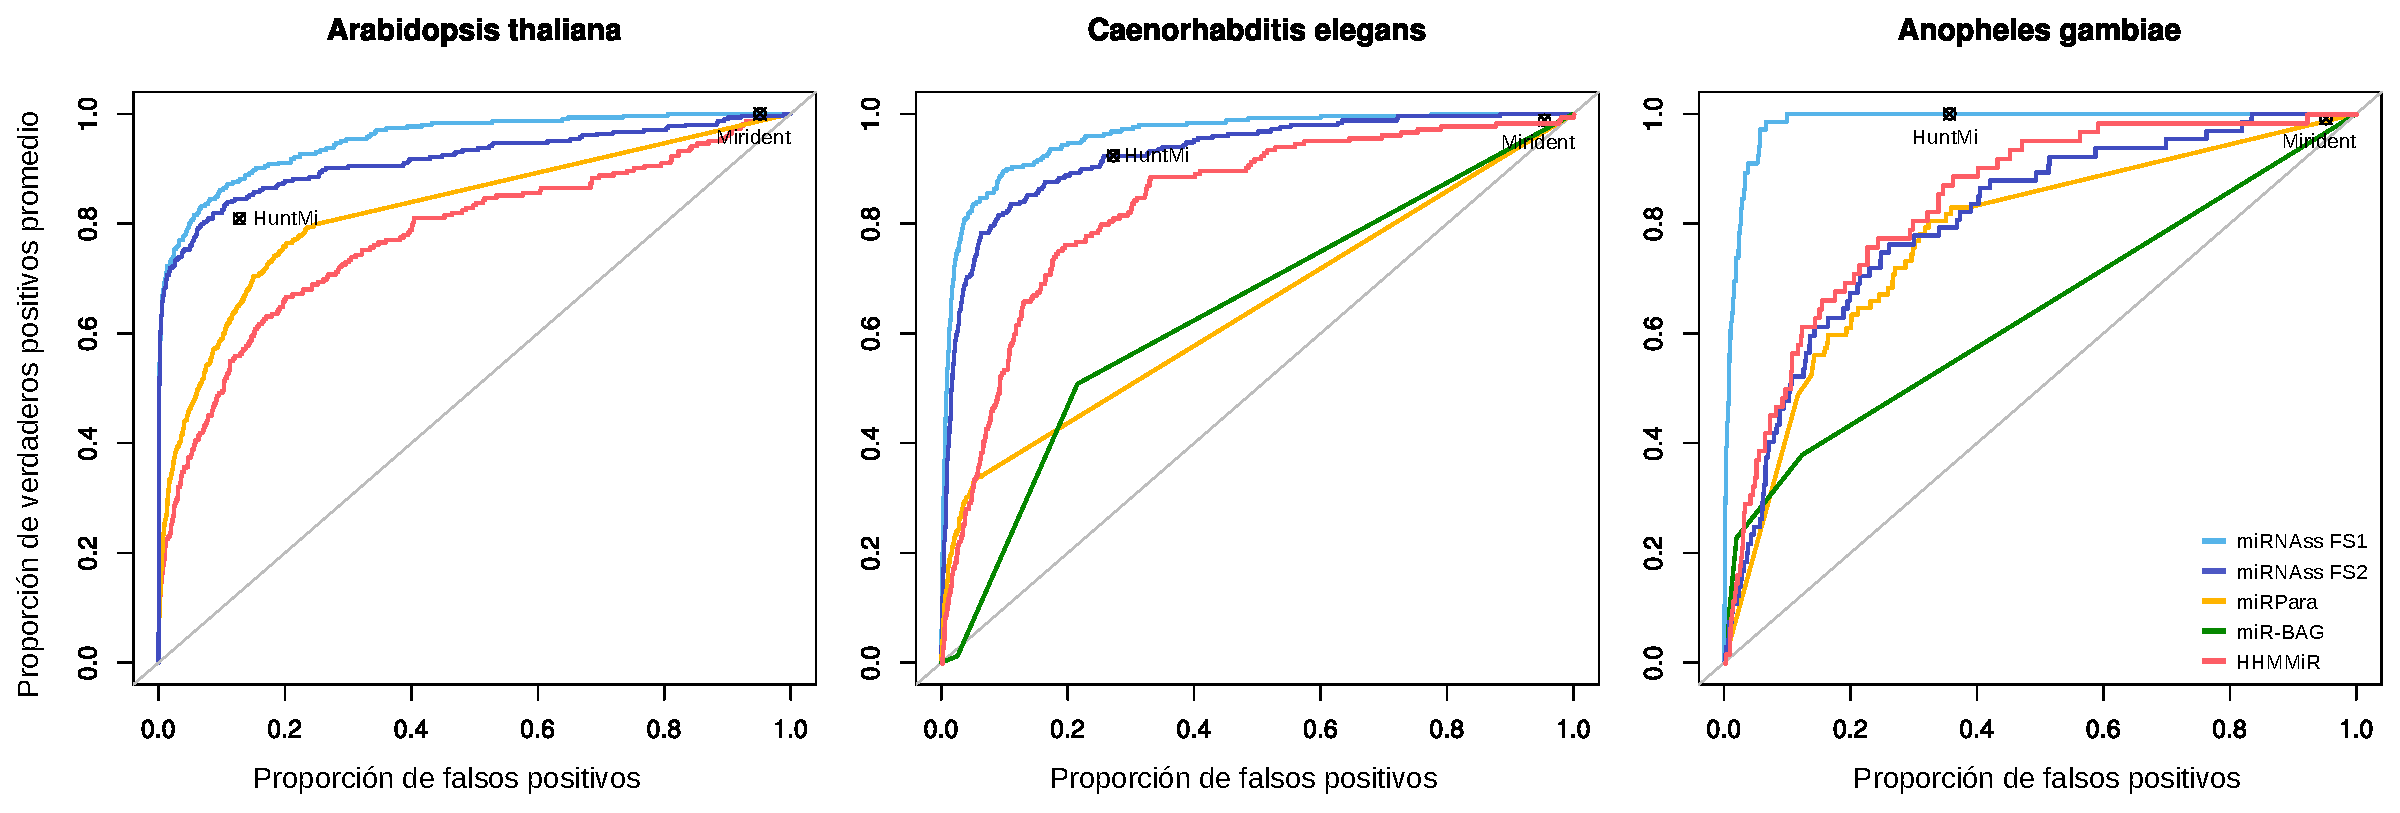
\includegraphics[width=\linewidth]{fig/genome-wide_ROC.eps}
	\caption[Curvas ROC en genoma completo]{Curvas ROC de miRNAss y otros métodos del estado del arte en datos de genoma completo de tres especies. Los puntos muestran el desempeño
		alcanzado por los métodos que generan clasificaciones sin puntajes de predicción.}
	\label{fig:ROC}
\end{figure*}
En el caso del genoma de \textit{A. gambiae}, el rendimiento de miRNAss con FS1 es más distante al obtenido con FS2. MiR-BAG y HHMMiR generan una curva
similar a la obtenida por miRNAss con FS2, muy por debajo de la obtenida con FS1. La curva ROC con FS1 muestra, en la esquina superior izquierda, que miRNAss
puede proporcionar el mejor equilibrio entre sensibilidad y tasa de falsos positivos. De hecho, esta es casi una curva ROC ideal.

Finalmente, como resumen del análisis comparativo, la Tabla~\ref{tab:wholegenome} presenta más resultados de interés práctico. Los mismos métodos y
especies de la Figura~\ref{fig:ROC} se analizan aquí según el rendimiento global y el número total de candidatos que devuelve cada método utilizando sus
valores de umbral predeterminados, es decir, la suma de verdaderos positivos y falsos positivos ( $TPFP$). Se puede ver que miARNs supera a todos los métodos
en los tres genomas. Mirident es el método con el rendimiento más bajo para todas las especies. Esto se debe a que etiqueta como positivos casi todos los
ejemplos, lo que se refleja en una sensibilidad muy alta, pero sin utilidad práctica dada la cantidad de candidatos proporcionados. MiR-BAG tiene un mejor
pero aún pobre desempeño en ambas especies. HHMMiR y miRPara predicen muy pocos candidatos, con alta especificidad a costa de una sensibilidad muy baja.
HuntMi, en cambio, permite obtener resultados más equilibrados, con el segundo mejor rendimiento. Sin embargo, en \textit{A. gambiae} devuelve una cantidad de
falsos positivos más de 5 veces mayor que los devueltos por miRNAss.

Estos resultados nos permiten afirmar que miRNAss supera a los métodos supervisados en una configuración de clasificación realista.Los ejemplos
negativos definidos artificialmente se usan para entrenar modelos supervisados y, dado que estos ejemplos no son representativos de la gran diversidad de
la clase negativa, los modelos no descartan correctamente secuencias que no sean miARN. Por el contrario, miRNAss puede aprovechar mejor el gran número de
secuencias no etiquetadas para ajustarse mejor al límite de decisión alrededor de los pre-miARN, descartando el resto de las secuencias.

\begin{table}[tpb]
	\footnotesize
	\centering
	\caption[Resultados en genomá completo]{media geométrica de la sensibilidad y la especificidad ($\bar{G}$) y suma de falsos y verdaderos positivos 
		($TPFP$, por sus siglas en ingles) en las tres pruebas de genoma completo.
	\label{tab:wholegenome}}
	\begin{tabular}{@{}lrcrcrc@{}} \toprule
		&	\multicolumn{2}{c}{\textit{A. thaliana}}
		&	\multicolumn{2}{c}{\textit{C. elegans}}
		&	\multicolumn{2}{c}{\textit{A. gambiae}} \\
		\multirow{2}{*}{Classifier}	&	 $TPFP$		&	 $\bar{G}$
						&	 $TPFP$			&	 $\bar{G}$
						&	 $TPFP$			&	 $\bar{G}$	\\\midrule
		{\small Mirident}	&	 1,294,648		&	 22.05 \%
					&	 1,617,221		&	 21.29 \%
					&	 4,068,431		&	 21.86 \%	\\
		{\small miR-BAG}	&	 -			&	 -
					&	 375,011		&	 63.14 \%
					&	 495,231		&	 57.62 \%	\\
		{\small miRPara}	&	 2,755			&	 47.95 \%
					&	 11,712			&	 53.79 \%
					&	 283,232		&	 72.48 \%	\\
		{\small HHMMiR}		&	 45,104			&	 69.07 \%
					&	 40,318			&	 73.29 \%
					&	 91,093			&	 74.07 \%	\\
		{\small HuntMi}		&	 173,906		&	 84.00 \%
					&	 462,203		&	 82.00 \%
					&	 1,456,590		&	 80.20 \%	\\
		{\small MiRNAss}	&	134,369		&	\textbf{84.82 \%}
					&	 164,557		&	 \textbf{87.61 \%}
					&	 258,096		&	 \textbf{93.34 \%}	\\\bottomrule
	\end{tabular}
\end{table}
